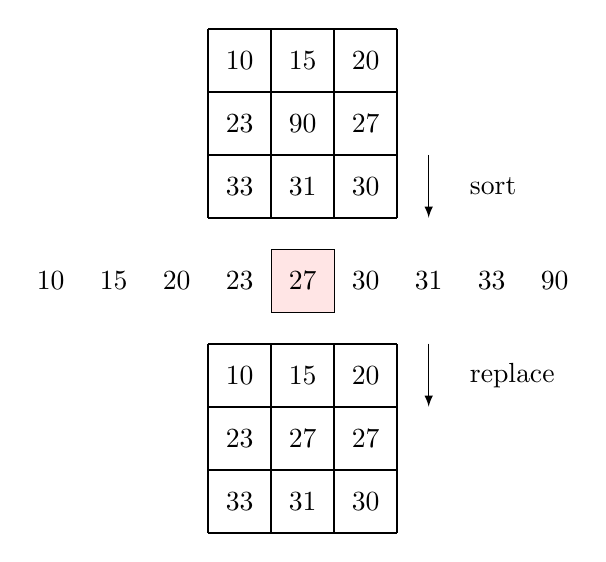
\begin{tikzpicture}[scale=0.8]

\draw [thick, step=1cm] (0,0) grid (3,3);
\foreach \i/\v in {0/33, 1/31, 2/30, 3/23, 4/90, 5/27,6/10, 7/15, 8/20}
{	
	\pgfmathparse{round(mod(\i,3)) + 0.5};
	\let\x\pgfmathresult;
	\pgfmathparse{round(div(\i,3)) + 0.5};
	\let\y\pgfmathresult;	
	\node at (\x, \y) {\v};
}
\draw[-latex] (3.5, 1) -- ++(0,-1);
\node [anchor=west] at (4, 0.5) {sort};

\draw[fill=red!10] (1, -1.5) rectangle ++(1,1);
\foreach \i/\v in {0/10, 1/15, 2/20, 3/23, 4/27, 5/30, 6/31, 7/33, 8/90}
{
	\node at (-2.5 + \i, -1) {\v};
}



\draw[-latex] (3.5, -2) -- ++(0,-1);
\node [anchor=west] at (4, -2.5) {replace};


\draw [thick, step=1cm] (0,-5) grid++ (3,3);
\foreach \i/\v in {0/33, 1/31, 2/30, 3/23, 4/27, 5/27,6/10, 7/15, 8/20}
{	
	\pgfmathparse{round(mod(\i,3)) + 0.5};
	\let\x\pgfmathresult;
	\pgfmathparse{round(div(\i,3)) + 0.5 -5};
	\let\y\pgfmathresult;	
	\node at (\x, \y) {\v};
}
\end{tikzpicture}